\chapter{Spéciation et macroévolution}\label{ch:b2:speciation}

Sur une petite île des Galápagos, en 1982, quelques géospizes à gros bec
arrivèrent d'une île voisine et s'y installèrent. Pendant vingt ans, ils
furent en compétition avec le géospize à bec moyen résident pour les
grosses \omterm{def:b2:angiosperm-reproduction:seed}{graines} que les deux espèces préféraient~; puis vint une
sécheresse, les grosses \omterm{def:b2:angiosperm-reproduction:seed}{graines} se raréfièrent, et les résidents aux becs
les plus gros --- ceux qui entraient le plus directement en compétition
avec les nouveaux venus --- moururent de faim. En une génération, les becs
des résidents avaient rétréci, de façon mesurable, en s'éloignant de ceux
des envahisseurs. Deux espèces qui s'étaient rencontrées avaient été
écartées l'une de l'autre. Ce chapitre traite de la formation des
espèces~: ce qu'est une espèce et ce qui la maintient distincte, comment
une population en devient deux, la compétition qui écarte les populations
lorsqu'elles se rencontrent, et la vision à long terme des archives
fossiles, où le même processus répété plus de cent millions de fois
donne l'arbre du vivant.

\section{Ce qu'est une espèce}

\begin{definition}[Espèce]\label{def:b2:speciation:species}
\index{concept d'espece@concept d'espèce}\index{concept biologique de l'espece@concept biologique de l'espèce}\index{isolement reproducteur}
Selon le \emph{concept biologique de l'espèce}, une espèce est un groupe
de populations dont les membres peuvent se croiser entre eux et
produire une descendance féconde, et qui sont \emph{isolées
reproductivement} des autres groupes de ce type~: ce qui unit une espèce,
c'est le \omterm{prop:b2:population-genetics:migration}{flux génique}, et ce qui sépare les espèces, c'est son absence.
Le concept fonctionne pour les organismes sexués d'un même temps et d'un
même lieu, qui constituent l'essentiel de ce que rencontre un
biologiste~; il échoue pour les lignées asexuées (que l'on nomme d'après
leur ressemblance), pour les fossiles (que l'on ne peut pas croiser), et
pour les nombreux cas où la frontière est poreuse --- chênes et saules
qui s'hybrident entre espèces, canards dont les espèces se croisent en
captivité, espèces en anneau dans lesquelles les populations voisines se
croisent tout autour d'une barrière jusqu'à ce que les extrémités se
rejoignent et ne se croisent plus. D'autres concepts comblent ces lacunes~:
l'espèce \emph{morphologique} (un groupe de formes semblables), l'espèce
\emph{phylogénétique} (la plus petite lignée diagnosable), l'espèce
\emph{écologique} (une lignée qui occupe sa propre niche). Aucun n'est
faux~; chacun mesure quelque chose de réel, et la spéciation est le
processus par lequel ils finissent par concorder.
\end{definition}

\begin{proposition}[Les mécanismes d'isolement]\label{prop:b2:speciation:isolation}
\index{mecanisme d'isolement@mécanisme d'isolement}\index{isolement prezygotique@isolement prézygotique}\index{isolement postzygotique}\index{regle de Haldane@règle de Haldane}
Le \omterm{prop:b2:population-genetics:migration}{flux génique} entre deux populations est arrêté par des barrières qui
agissent avant ou après la fécondation. \emph{Prézygotiques}~: les
populations vivent dans des habitats différents ou se reproduisent à des
saisons différentes (isolement temporel~: deux grenouilles qui chantent à
des mois différents)~; elles ne reconnaissent pas la parade l'une de
l'autre (isolement comportemental~: les chants des grillons, les codes
lumineux des lucioles, les parades des canards)~; leurs organes génitaux
ou leurs \omterm{def:b2:angiosperm-reproduction:flower}{fleurs} ne s'ajustent pas (isolement mécanique)~; leurs gamètes
ne fusionnent pas (isolement gamétique~: les protéines de fixation du
spermatozoïde des oursins, les \omterm{def:b2:meiosis-heredity:vocabulary}{allèles}
$S$ du \cref{ch:b2:angiosperm-reproduction}).
\emph{Postzygotiques}~: l'hybride meurt à l'état d'embryon, ou vit mais
est stérile (le mulet~; les hybrides de deux espèces de \emph{Drosophila}),
ou est fertile mais sa propre descendance ne l'est pas (dégénérescence
des hybrides). \emph{\omterm{prop:b2:speciation:isolation}{Règle de Haldane}}~: lorsqu'un seul sexe d'un hybride
est stérile ou non viable, c'est le sexe qui porte deux \omterm{prop:b2:meiosis-heredity:sexlinked}{chromosomes
sexuels} différents --- le mâle chez les mammifères et les mouches, la
femelle chez les oiseaux et les papillons --- parce que les
incompatibilités récessives portées par le X y sont exposées. Les
barrières prézygotiques coûtent moins, puisqu'aucun gamète n'est gaspillé,
et la sélection les construit là où les barrières postzygotiques existent
déjà.
\end{proposition}

\begin{theorem}[Pourquoi les hybrides échouent~: le modèle à deux locus]\label{thm:b2:speciation:dm}
\index{incompatibilite de Dobzhansky--Muller@incompatibilité de Dobzhansky--Muller}
Deux populations partent du \omterm{def:b2:meiosis-heredity:vocabulary}{génotype} $aabb$. Dans l'une, $a$ est remplacé
par $A$~; dans l'autre, $b$ par $B$~; chaque substitution est neutre ou
favorable dans son propre fond génétique, si bien qu'aucune des deux
populations ne passe jamais par un état de moindre \omterm{def:b2:population-genetics:fitness}{valeur sélective}. Mais
$A$ et $B$ n'ont jamais été éprouvés ensemble, et si la combinaison est
incompatible --- si la protéine que fabrique $A$ ne peut pas fonctionner
avec la protéine que fabrique $B$ --- l'hybride $AaBb$ est désavantagé.
L'\omterm{def:b2:speciation:species}{isolement reproducteur} apparaît ainsi comme un sous-produit de la
divergence, sans vallée franchie et sans sélection en faveur de
l'isolement lui-même~; et comme chaque nouvelle substitution dans une
lignée peut être incompatible avec chacune des substitutions déjà fixées
dans l'autre, le nombre d'incompatibilités possibles croît comme le
\emph{carré} du nombre de substitutions --- l'isolement fait \emph{boule
de neige} avec le temps.
\end{theorem}
\begin{proof}
Avec $n$ substitutions dans chaque lignée, chacun des $n$ nouveaux \omterm{def:b2:meiosis-heredity:vocabulary}{allèles}
d'une lignée peut être incompatible avec chacun des $n$ \omterm{def:b2:meiosis-heredity:vocabulary}{allèles} de
l'autre~: $n^{2}$ paires, chacune incompatible avec une certaine probabilité
$\varepsilon$, si bien que le nombre attendu d'incompatibilités vaut
$\varepsilon n^{2}$, et $n$ croît avec le temps écoulé depuis la
séparation. L'hybride est le seul \omterm{def:b2:meiosis-heredity:vocabulary}{génotype} dans lequel les deux ensembles
se rencontrent.
\end{proof}
\begin{proof}[Faits expérimentaux]
Coyne et Orr (1989, 1997) compilèrent des centaines de paires d'espèces
de \emph{Drosophila} de distance génétique connue (une mesure du temps
écoulé depuis la divergence) et mesurèrent leur \omterm{prop:b2:speciation:isolation}{isolement prézygotique} et
postzygotique~: tous deux augmentent avec la distance, l'isolement est
pratiquement complet à une distance correspondant à quelques millions
d'années, et les paires qui vivent dans la même région montrent, à
distance égale, un \omterm{prop:b2:speciation:isolation}{isolement prézygotique} plus fort que les paires qui
vivent séparées --- la signature du renforcement. Les gènes
d'incompatibilité ont depuis été identifiés un à un, et leur nombre entre
deux espèces croît bien plus vite que linéairement avec la divergence.
\end{proof}

\begin{omfigure}
\begin{tikzpicture}[every node/.style={font=\scriptsize}, >=stealth]
  \node[draw, rounded corners, fill=omExo!25] (anc) at (0,0) {ancêtre $aabb$};
  \node[draw, rounded corners, fill=omDef!15] (p1) at (-2.6,-1.8) {population 1~: $AAbb$};
  \node[draw, rounded corners, fill=omThm!15] (p2) at (2.6,-1.8) {population 2~: $aaBB$};
  \node[draw, rounded corners, fill=gray!25, align=center] (hyb) at (0,-3.6) {hybride $AaBb$~:\\$A$ et $B$ se rencontrent pour la première fois\\--- incompatibles, désavantagé};
  \draw[->, thick] (anc) -- (p1) node[midway, left, align=right] {$a \to A$ fixé,\\favorable dans son fond};
  \draw[->, thick] (anc) -- (p2) node[midway, right, align=left] {$b \to B$ fixé,\\favorable dans son fond};
  \draw[->, thick] (p1) -- (hyb); \draw[->, thick] (p2) -- (hyb);
  \node[anchor=west, align=left, text width=4.6cm] at (4.6,-0.4) {aucune population n'a franchi de vallée~; l'isolement est un sous-produit, et le nombre de telles paires croît comme $n^{2}$};
\end{tikzpicture}

{\small Le modèle à deux locus de l'échec des hybrides. Chaque population
fixe un changement qui fonctionne dans son propre fond génétique~;
l'hybride est le premier \omterm{def:b2:meiosis-heredity:vocabulary}{génotype} qui combine les deux.}
\end{omfigure}

\section{Comment une espèce en devient deux}

\begin{proposition}[Les modes de spéciation]\label{prop:b2:speciation:modes}
\index{speciation allopatrique@spéciation allopatrique}\index{speciation sympatrique@spéciation sympatrique}\index{speciation parapatrique@spéciation parapatrique}\index{effet fondateur}
La spéciation \emph{allopatrique} commence par une barrière
géographique~: une aire de répartition coupée par une montagne qui
s'élève, une mer qui s'assèche ou un nouveau fleuve
(\emph{vicariance}), ou quelques colons emportés sur une île
(spéciation \emph{péripatrique}, avec l'\omterm{prop:b2:speciation:modes}{effet fondateur} et la dérive du
\cref{ch:b2:population-genetics} en prime). Coupées du \omterm{prop:b2:population-genetics:migration}{flux génique},
les deux populations divergent par la sélection dans des environnements
différents, par la dérive et par leurs \omterm{def:b2:genome-diversification:mutation}{mutations} propres, jusqu'à ce que
des incompatibilités se soient accumulées~; si elles se rencontrent de
nouveau, elles ne fusionnent plus. C'est le mode le plus commun, et la
répartition d'espèces sœurs de part et d'autre de chaque isthme, de
chaque chaîne de montagnes et de chaque détroit en est la trace.
La spéciation \emph{sympatrique} se produit sans barrière~: en une seule
étape par \omterm{def:b2:genome-diversification:polyploidy}{polyploïdie} (\cref{ch:b2:genome-diversification}) --- un tiers
des espèces végétales sont nées ainsi~; ou par sélection disruptive
accompagnée d'accouplements homogames, lorsqu'une population exploite
deux ressources et que les individus s'accouplent sur la ressource qu'ils
utilisent (la mouche de la pomme, passée de l'aubépine au pommier dans
les années 1860 et qui s'accouple aujourd'hui sur son hôte~; les cichlidés
d'un lac de cratère). La spéciation \emph{parapatrique} se produit le long
d'un gradient environnemental, où une population s'adapte aux deux
extrémités et où une \omterm{prop:b2:speciation:reinforcement}{zone hybride} se forme au milieu. Dans tous les
modes, la recette est la même~: réduire le \omterm{prop:b2:population-genetics:migration}{flux génique}, laisser la
divergence s'accumuler, et laisser les sous-produits de la divergence
devenir des barrières.
\end{proposition}

\begin{omfigure}
\resizebox{\linewidth}{!}{%
\begin{tikzpicture}[every node/.style={font=\scriptsize}, >=stealth]
  \foreach \x/\lab in {0/{allopatrique~:\\une barrière coupe l'aire}, 5.2/{péripatrique~:\\quelques fondateurs sur une île}, 10.4/{sympatrique~:\\deux hôtes, accouplement sur l'hôte}} \node[align=center, anchor=south] at (\x+1.8,3.0) {\lab};
  % allopatric
  \draw[thick, fill=omDef!15] (0.9,1.4) ellipse (0.8 and 0.9);
  \draw[thick, fill=omThm!15] (2.7,1.4) ellipse (0.8 and 0.9);
  \draw[very thick, omExo!70!black] (1.8,0.2) -- (1.8,2.6);
  \node[below] at (1.8,0.1) {montagne, mer, fleuve};
  % peripatric
  \begin{scope}[xshift=5.2cm]
    \draw[thick, fill=omDef!15] (1.0,1.4) ellipse (1.0 and 0.9);
    \draw[thick, fill=omThm!15] (3.2,1.9) circle (0.35);
    \draw[->, thick, dashed] (2.0,1.6) -- (2.85,1.85);
    \node[below] at (3.2,1.5) {fondateurs};
    \node[below] at (1.0,0.4) {continent};
  \end{scope}
  % sympatric
  \begin{scope}[xshift=10.4cm]
    \draw[thick, fill=omExo!15] (1.8,1.4) ellipse (1.7 and 0.9);
    \foreach \p in {(1.0,1.6),(1.3,1.2),(0.8,1.2),(1.2,1.8)} \fill[omDef] \p circle (0.07);
    \foreach \p in {(2.4,1.6),(2.7,1.2),(2.2,1.2),(2.6,1.8)} \fill[omThm] \p circle (0.07);
    \node[omDef, below] at (1.0,0.5) {hôte A}; \node[omThm, below] at (2.6,0.5) {hôte B};
    \node[below] at (1.8,0.1) {un lieu, deux ressources};
  \end{scope}
\end{tikzpicture}}

{\small Trois chemins vers deux espèces~: une barrière qui traverse l'aire
de répartition, une population fondatrice au-delà, ou deux ressources
en son sein.}
\end{omfigure}

\begin{proposition}[Renforcement et zones hybrides]\label{prop:b2:speciation:reinforcement}
\index{renforcement}\index{zone hybride}\index{cline}
Lorsque deux populations qui ont divergé se rencontrent de nouveau, trois
choses peuvent arriver. Si leurs hybrides ont la même \omterm{def:b2:population-genetics:fitness}{valeur sélective} que
les parents, elles fusionnent. Si les hybrides sont désavantagés, la
sélection favorise les individus qui refusent de s'accoupler avec l'autre
forme --- les gamètes gaspillés sont le coût --- et l'\omterm{prop:b2:speciation:isolation}{isolement
prézygotique} se renforce là où les deux se chevauchent
(\emph{renforcement}), jusqu'à ce qu'elles soient des espèces. Entre ces
deux cas, une \emph{\omterm{prop:b2:speciation:reinforcement}{zone hybride}} persiste~: une bande, souvent large de
quelques kilomètres, où les deux formes se croisent et où des hybrides
sont produits à chaque génération, maintenue par l'équilibre entre la
dispersion vers la zone et la sélection contre les hybrides qui s'y
trouvent. À travers une telle zone, la fréquence de chaque forme suit un
\emph{cline}, une courbe en S dont la largeur $w$ est fixée par la
distance de dispersion $\sigma$ par génération et la sélection $s$ contre
les hybrides, $w \approx
\sigma\sqrt{8/s}$~: une zone peut rester étroite pendant des milliers
d'années sans que les deux formes fusionnent jamais ni se séparent
complètement. Les crapauds, les corneilles, les souris et les criquets
d'Europe en montrent des dizaines, la plupart situées le long des lignes
où des populations qui s'étaient abritées dans des refuges séparés
pendant la dernière glaciation se sont rencontrées de nouveau lors du
retrait des glaces.
\end{proposition}
\begin{proof}[Faits expérimentaux]
Là où le gobemouche noir et le gobemouche à collier se chevauchent, en
Europe centrale, les mâles de chaque espèce ont un plumage plus différent
de celui de l'autre que là où ils vivent séparés, et les femelles
discriminent plus nettement --- le renforcement mesuré sur le terrain.
Le sonneur à ventre de feu et le sonneur à ventre jaune se rencontrent le
long d'une zone qui traverse la Pologne, large de quelques kilomètres,
stable depuis qu'elle est étudiée, avec la largeur de cline prédite à
partir de leur dispersion et de la \omterm{def:b2:population-genetics:fitness}{valeur sélective} réduite de leurs
hybrides.
\end{proof}

\begin{omfigure}
\begin{tikzpicture}
\begin{axis}[
  width=0.72\linewidth, height=5.2cm,
  axis x line=bottom, axis y line=left,
  xmin=-30, xmax=30, ymin=0, ymax=1.05,
  xlabel={distance à travers la zone (km)}, ylabel={fréquence de la forme A},
  xlabel style={font=\small, at={(axis description cs:0.5,-0.13)}, anchor=north},
  ylabel style={font=\small},
  tick label style={font=\small}, xtick={-20,-10,0,10,20}, ytick={0,0.5,1},
  clip=false,
]
\addplot[very thick, omDef, domain=-30:30, samples=100] {1/(1+exp(x/2.2))};
\draw[dashed, gray] (axis cs:-4.4,0) -- (axis cs:-4.4,1); \draw[dashed, gray] (axis cs:4.4,0) -- (axis cs:4.4,1);
\draw[<->] (axis cs:-4.4,0.08) -- (axis cs:4.4,0.08); \node[font=\scriptsize, anchor=south] at (axis cs:0,0.09) {largeur $w$};
\node[font=\scriptsize, anchor=west, align=left] at (axis cs:8,0.75) {$w \approx \sigma\sqrt{8/s}$~: une dispersion\\$\sigma = \qty{1}{km}$ et $s = 0.1$\\donnent $w \approx \qty{9}{km}$};
\end{axis}
\end{tikzpicture}

{\small Un cline à travers une \omterm{prop:b2:speciation:reinforcement}{zone hybride}~: la fréquence d'une forme
passe de un à zéro sur une largeur fixée par la distance de dispersion
des individus et par le désavantage de leurs hybrides.}
\end{omfigure}

\section{Compétition, coexistence et déplacement de caractère}

\begin{theorem}[La compétition de Lotka--Volterra]\label{thm:b2:speciation:lv}
\index{competition de Lotka--Volterra@compétition de Lotka--Volterra}\index{exclusion competitive@exclusion compétitive}\index{coexistence}
Deux espèces à croissance logistique (volume de première année) en
compétition pour une ressource obéissent à
\[
\frac{\mathrm{d}N_1}{\mathrm{d}t} = r_1 N_1\Bigl(1 - \frac{N_1 + \alpha N_2}{K_1}\Bigr), \qquad
\frac{\mathrm{d}N_2}{\mathrm{d}t} = r_2 N_2\Bigl(1 - \frac{N_2 + \beta N_1}{K_2}\Bigr),
\]
où $\alpha$ mesure l'effet d'un individu de l'espèce 2 sur l'espèce 1,
en unités d'individus de l'espèce 1, et $\beta$
l'effet inverse. L'espèce 1 cesse de croître sur la droite $N_1 + \alpha N_2 =
K_1$ (son \emph{isocline}), l'espèce 2 sur $N_2 + \beta N_1 = K_2$, et
l'issue dépend de la manière dont les deux droites se coupent~:
\begin{itemize}
  \item $K_1 > \alpha K_2$ et $K_2 < \beta K_1$~: l'espèce 1 l'emporte
        toujours~;
  \item $K_1 < \alpha K_2$ et $K_2 > \beta K_1$~: l'espèce 2 l'emporte
        toujours~;
  \item $K_1 > \alpha K_2$ et $K_2 > \beta K_1$~: \emph{coexistence
        stable} en $N_1^{*} = (K_1 - \alpha K_2)/(1 - \alpha\beta)$,
        $N_2^{*} = (K_2 - \beta K_1)/(1 - \alpha\beta)$~;
  \item $K_1 < \alpha K_2$ et $K_2 < \beta K_1$~: l'une ou l'autre
        l'emporte, selon celle qui part la plus nombreuse.
\end{itemize}
La coexistence exige $\alpha\beta < 1$, chaque espèce étant davantage
limitée par ses propres congénères que par l'autre~: deux espèces qui
utilisent exactement la même ressource ($\alpha = \beta = 1$) ne peuvent
pas coexister (le \emph{principe d'\omterm{thm:b2:speciation:lv}{exclusion compétitive}}), et plus
elles diffèrent dans ce qu'elles utilisent, plus $\alpha$ et $\beta$ sont
petits et plus leur coexistence est assurée.
\end{theorem}
\begin{proof}
Sur l'isocline de l'espèce 1, $\mathrm{d}N_1/\mathrm{d}t = 0$~; en dessous
(vers l'origine), $N_1$ croît, au-dessus, $N_1$ décroît~; de même pour
l'espèce 2. Chaque isocline est une droite d'ordonnées à l'origine $K_1$
sur l'axe $N_1$ et $K_1/\alpha$ sur l'axe $N_2$ (pour l'espèce 1),
$K_2/\beta$ et $K_2$ (pour l'espèce 2). L'espèce 1 peut envahir une
population de l'espèce 2 à sa capacité de charge $K_2$ si sa propre
croissance y est positive, c'est-à-dire si $K_1 > \alpha K_2$~; l'espèce 2
peut envahir l'espèce 1 à $K_1$ si $K_2 > \beta K_1$. Lorsque chacune peut
envahir l'autre, aucune ne peut être exclue et les trajectoires
convergent vers le croisement des isoclines, obtenu en résolvant les
équations des deux droites~; lorsqu'une seule le peut, elle l'emporte~;
lorsqu'aucune ne le peut, le croisement est un col et la première
installée l'emporte. La stabilité du point intérieur découle de
l'argument d'invasion~: écartée vers l'un ou l'autre axe, l'espèce devenue
rare croît de nouveau.
\end{proof}

\begin{omfigure}
\begin{tikzpicture}
\begin{axis}[
  width=0.6\linewidth, height=6cm,
  axis x line=bottom, axis y line=left,
  xmin=0, xmax=1300, ymin=0, ymax=1900,
  xlabel={$N_1$}, ylabel={$N_2$},
  xlabel style={font=\small, at={(axis description cs:0.5,-0.1)}, anchor=north},
  ylabel style={font=\small},
  tick label style={font=\small}, xtick={0,857,1000,1333}, xticklabels={0,$N_1^*$,$K_1$,$K_2/\beta$}, ytick={0,286,800,2000}, yticklabels={0,$N_2^*$,$K_2$,$K_1/\alpha$},
  clip=false,
]
\addplot[very thick, omDef, domain=50:1000, samples=2] {(1000-x)/0.5};
\addplot[very thick, omThm, domain=0:1333, samples=2] {800-0.6*x};
\fill[black] (axis cs:857,286) circle (2.5pt);
\draw[->, thick, gray] (axis cs:150,1750) -- (axis cs:300,1450);
\draw[->, thick, gray] (axis cs:1200,100) -- (axis cs:1000,250);
\draw[->, thick, gray] (axis cs:150,150) -- (axis cs:400,250);
\node[font=\scriptsize, omDef, anchor=west] at (axis cs:700,1000) {isocline de l'espèce 1};
\node[font=\scriptsize, omThm, anchor=south west] at (axis cs:130,740) {isocline de l'espèce 2};
\node[font=\scriptsize, anchor=south west] at (axis cs:880,320) {coexistence stable};
\end{axis}
\end{tikzpicture}

{\small Le plan de phase de deux compétiteurs avec $K_1 = 1000$, $K_2 =
800$, $\alpha = 0.5$, $\beta = 0.6$~: chaque espèce peut envahir l'autre
à sa capacité de charge, et les trajectoires convergent vers le
croisement des isoclines, en $N_1^{*} = 857$, $N_2^{*} = 286$.}
\end{omfigure}

\begin{proposition}[Le déplacement de caractère]\label{prop:b2:speciation:displacement}
\index{deplacement de caractere@déplacement de caractère}\index{niche}\index{radiation adaptative}
La compétition n'est pas seulement une issue écologique mais une force
évolutive. Là où deux espèces semblables se rencontrent, les individus de
chacune qui ressemblent le plus à l'autre souffrent le plus de la
compétition, et la sélection écarte les deux espèces pour le caractère
qui gouverne l'utilisation de la ressource --- la taille du bec, la
taille du corps, l'époque de floraison~: les populations qui se
chevauchent diffèrent davantage que les populations qui vivent
seules. Ce \emph{\omterm{prop:b2:speciation:displacement}{déplacement de caractère}} réduit $\alpha$ et
$\beta$, change une lutte d'exclusion en coexistence, et, répété sur un
paysage d'opportunités, produit une
\emph{\omterm{prop:b2:speciation:displacement}{radiation adaptative}}~: un colon unique devenant une douzaine
d'espèces, chacune ajustée à une ressource --- les pinsons de Darwin aux
Galápagos, les drépanis d'Hawaï, les cichlidés des lacs africains
(cinq cents espèces dans le lac Victoria en moins de quinze mille ans),
les anolis des Caraïbes, chez lesquels le même ensemble de niches a été
occupé par le même ensemble de formes corporelles, indépendamment, sur
quatre îles.
\end{proposition}
\begin{proof}[Faits expérimentaux]
Les Grant recensèrent chaque pinson de Daphne Major pendant quarante ans.
Après l'installation du géospize à gros bec en 1982, le bec du géospize à
bec moyen ne changea pas jusqu'à la sécheresse de 2004, lorsque les
grosses \omterm{def:b2:angiosperm-reproduction:seed}{graines} se raréfièrent et que les deux espèces se les
disputèrent~; les géospizes à bec moyen dont les becs étaient les plus
gros moururent en proportion excessive, et les becs de la génération
suivante étaient plus petits d'un écart jamais observé en une seule
étape --- le \omterm{prop:b2:speciation:displacement}{déplacement de caractère} prédit par la théorie, observé en
direct, avec sa différentielle de sélection et son héritabilité
mesurées. Les becs de ces mêmes pinsons, comparés entre les îles où ils
vivent seuls et celles où ils se rencontrent, montrent le même
déplacement inscrit à l'échelle de l'archipel.
\end{proof}

\begin{omfigure}
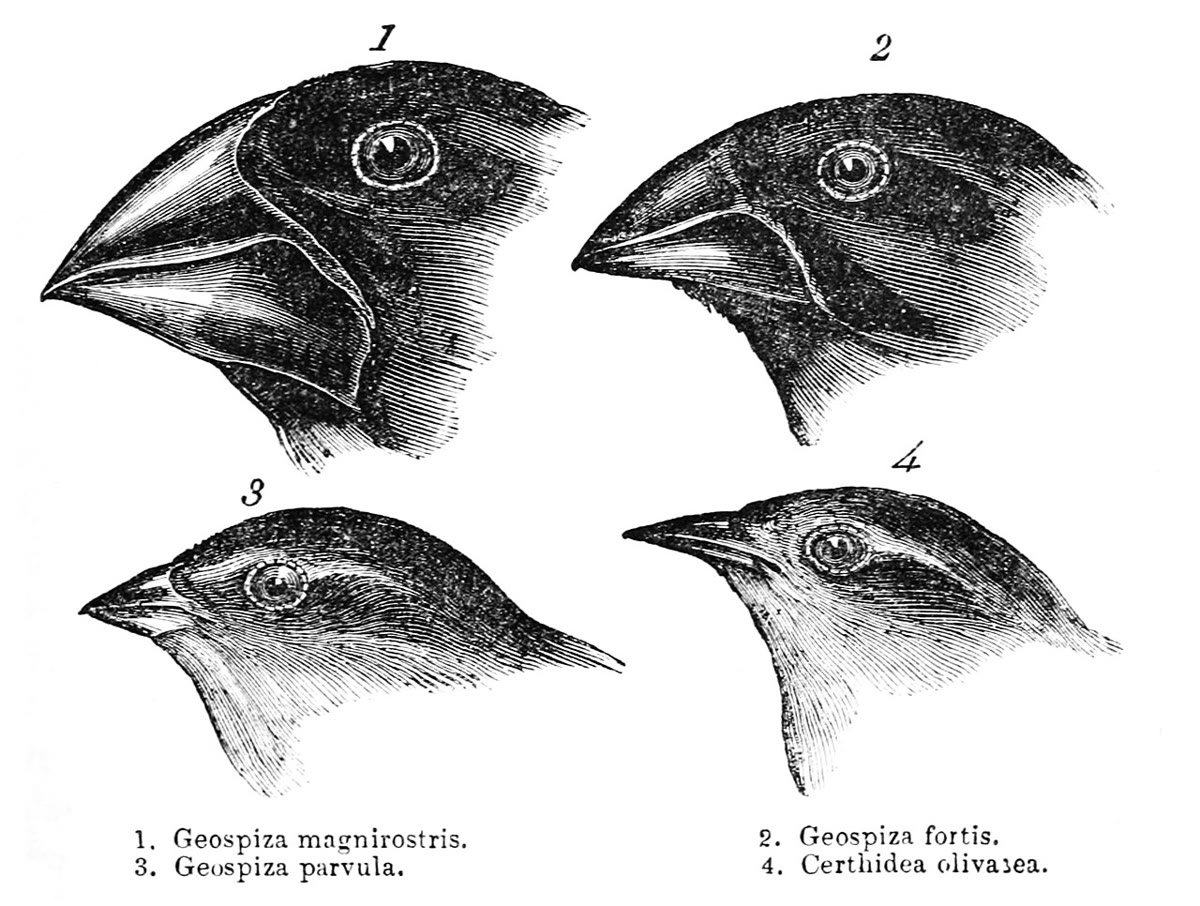
\includegraphics[width=0.44\linewidth]{images/book2/finches-gould.jpg}\hspace{0.04\linewidth}
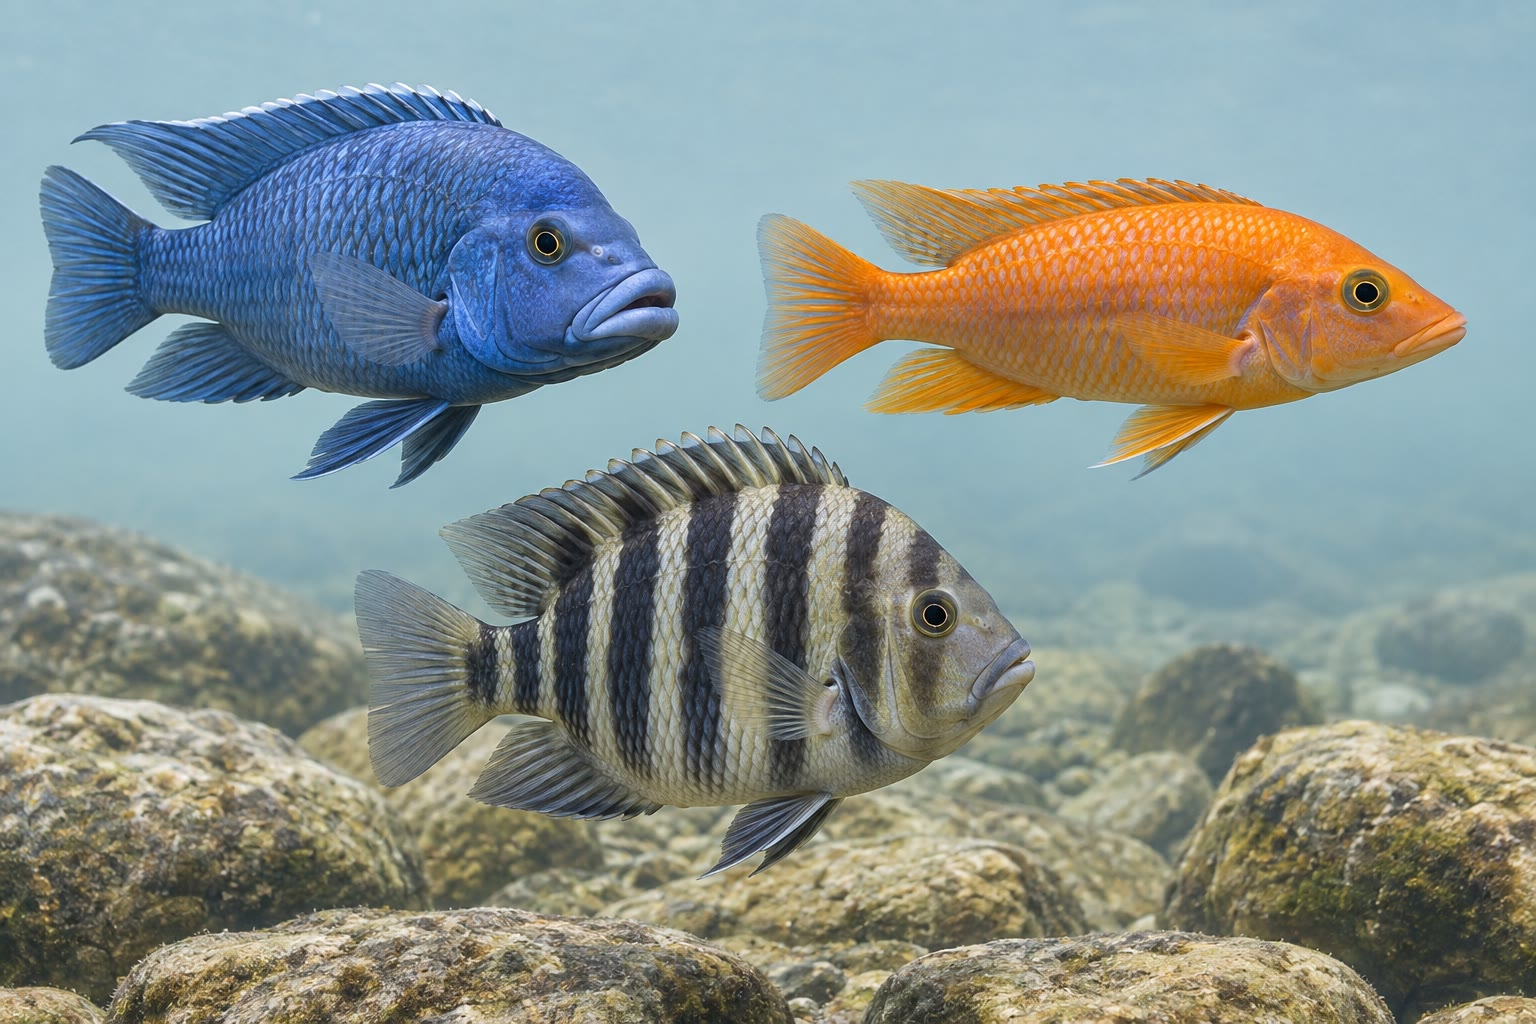
\includegraphics[width=0.44\linewidth]{images/book4/ai/b4-23-cichlids.jpg}

{\small Deux radiations. À gauche~: les pinsons de Darwin dessinés par
Gould en 1845, un colon devenu multiple, les espèces se distinguant par
leur bec. À droite~: des cichlidés d'un lac africain, des centaines
d'espèces issues de quelques fondateurs, chacune avec sa bouche et son
régime alimentaire.}
\end{omfigure}

\section{Macroévolution~: la vision à long terme}

\begin{proposition}[Tempo et mode]\label{prop:b2:speciation:tempo}
\index{equilibre ponctue@équilibre ponctué}\index{gradualisme}\index{extinction de masse}
En quelques dizaines de générations, la phalène a changé de couleur et le
pinson de bec~; sur des millions d'années, les archives fossiles montrent
des lignées qui changent à peine pendant de longues périodes puis, en un
instant géologique de quelques milliers d'années, sont remplacées par un
descendant distinct --- l'\emph{\omterm{prop:b2:speciation:tempo}{équilibre ponctué}}, qui est l'aspect que
prend une \omterm{prop:b2:speciation:modes}{spéciation allopatrique} dans de petites populations
périphériques suivie de leur expansion lorsqu'on l'échantillonne tous les
cent mille ans~; et elles montrent d'autres lignées, dont celle des
chevaux, qui changent graduellement au fil de dizaines d'espèces.
Au-dessus de l'espèce, les archives sont celles d'un renouvellement~: la
plupart des espèces durent de un à dix millions d'années, le taux
d'\emph{extinction de fond} est d'environ une espèce sur un
million par an, et à cinq reprises --- à la fin de l'Ordovicien, du
Dévonien, du Permien (lorsque les neuf dixièmes des espèces marines
disparurent), du Trias et du Crétacé --- une \emph{\omterm{prop:b2:speciation:tempo}{extinction de masse}} a
éliminé l'essentiel de ce qui vivait en quelques centaines de milliers
d'années et redistribué les cartes, les survivants rayonnant dans les
niches vidées~: les mammifères dans le monde des dinosaures après
l'astéroïde d'il y a 66 millions d'années. La macroévolution est le
motif qu'a dessiné la microévolution de ce chapitre et du précédent,
prolongée pendant très longtemps et interrompue par des catastrophes.
\end{proposition}

\begin{example}[Des vitesses comparées]\label{ex:b2:speciation:rates}
La sélection a modifié la hauteur du bec des pinsons de \qty{4}{\%} en une
génération~; la radiation entière des Galápagos, quatorze espèces issues
d'un fondateur, a pris deux millions d'années~; la différence de taille
corporelle entre une souris et un éléphant, un facteur de quelque
$10^{5}$, pourrait être produite par une sélection de l'intensité de
celle des pinsons en quelques centaines de générations ---
et les archives montrent qu'elle a pris quarante millions d'années. Le
paradoxe se résout en remarquant que la sélection pousse rarement
longtemps dans le même sens~: elle s'inverse avec le temps qu'il fait,
comme sur Daphne Major l'année qui suivit la sécheresse, et la \omterm{prop:b2:population-genetics:kinds}{sélection
stabilisante} maintient la plupart des lignées là où elles sont. Le
changement soutenu est rare, c'est pourquoi la spéciation, qui en a
besoin, est lente --- et c'est pourquoi, lorsque le monde change vite,
comme au \cref{ch:b2:global-change}, les lignées qui ne peuvent pas suivre
disparaissent.
\end{example}

\section{Exercices}

\begin{exercise}[$\star$]\label{exo:b2:speciation:1}
Énoncer le \omterm{def:b2:speciation:species}{concept biologique de l'espèce} et donner trois cas où il ne
peut pas s'appliquer, avec le concept utilisé à la place.
\end{exercise}

\begin{exercise}[$\star$]\label{exo:b2:speciation:2}
Classer comme prézygotique ou postzygotique~: deux grenouilles qui se
reproduisent à des mois différents~; un mulet~; un spermatozoïde d'oursin
qui ne peut pas se fixer sur le gamète femelle d'une autre espèce~; des plantes
hybrides vigoureuses mais dont les \omterm{def:b2:angiosperm-reproduction:seed}{graines} ne germent pas~; deux grillons
aux chants différents.
\end{exercise}

\begin{exercise}[$\star$]\label{exo:b2:speciation:3}
Définir les \omterm{prop:b2:speciation:modes}{spéciations allopatrique}, péripatrique, sympatrique et
parapatrique, avec un exemple de chacune.
\end{exercise}

\begin{exercise}[$\star$]\label{exo:b2:speciation:4}
Énoncer les quatre issues de la \omterm{thm:b2:speciation:lv}{compétition de Lotka--Volterra} et, en
mots, la condition de coexistence stable.
\end{exercise}

\begin{exercise}[$\star\star$]\label{exo:b2:speciation:5}
Avec $K_1 = 1000$, $K_2 = 800$, $\alpha = 0.5$, $\beta = 0.6$,
calculer les densités d'équilibre et vérifier que chaque espèce peut
envahir l'autre à sa capacité de charge.
\end{exercise}

\begin{exercise}[$\star\star$]\label{exo:b2:speciation:6}
Avec $K_1 = 1000$, $K_2 = 800$, $\alpha = 1.5$, $\beta = 0.3$, quelle
espèce l'emporte, et pourquoi~? Et si $\alpha = 1.5$ et $\beta = 1.5$~?
\end{exercise}

\begin{exercise}[$\star\star$]\label{exo:b2:speciation:7}
Un tétraploïde apparaît dans une population \omterm{def:b2:meiosis-heredity:meiosis}{diploïde}. Donner les nombres
chromosomiques de ses gamètes, d'un croisement avec le \omterm{def:b2:meiosis-heredity:meiosis}{diploïde} et des
gamètes de cet hybride, et expliquer pourquoi le tétraploïde est
immédiatement isolé. Pourquoi, néanmoins, ne se maintient-il
généralement pas~?
\end{exercise}

\begin{exercise}[$\star\star$]\label{exo:b2:speciation:8}
Deux populations ont chacune fixé 10 substitutions depuis leur
séparation, et chaque paire de nouveaux \omterm{def:b2:meiosis-heredity:vocabulary}{allèles} des deux côtés est
incompatible avec la probabilité $0.01$. Calculer le nombre attendu
d'incompatibilités aujourd'hui, et après 30 substitutions chacune.
Qu'est-ce que cela prédit pour la relation entre isolement et temps~?
\end{exercise}

\begin{exercise}[$\star\star$]\label{exo:b2:speciation:9}
Calculer la largeur d'une \omterm{prop:b2:speciation:reinforcement}{zone hybride} pour une dispersion $\sigma =
\qty{2}{km}$ par génération et un désavantage des hybrides $s = 0.05$, et
pour $\sigma = \qty{0.3}{km}$ et $s = 0.4$. Quelle zone a le plus de
chances d'aboutir à un renforcement, et pourquoi~?
\end{exercise}

\begin{exercise}[$\star\star\star$]\label{exo:b2:speciation:10}
Deux espèces de pinsons sont en compétition pour les \omterm{def:b2:angiosperm-reproduction:seed}{graines} avec
$\alpha = \beta = 0.9$ et
$K_1 = K_2 = 500$. Coexistent-elles~? Le \omterm{prop:b2:speciation:displacement}{déplacement de caractère} réduit
$\alpha$ et $\beta$ à $0.4$~: recalculer l'équilibre. Expliquer, en
termes d'isoclines, ce qu'a produit le déplacement.
\end{exercise}

\begin{exercise}[$\star\star\star$]\label{exo:b2:speciation:11}
Les Grant ont trouvé qu'après la sécheresse de 2004 la hauteur moyenne
du bec du géospize à bec moyen avait diminué de \qty{0.7}{mm}, avec
$h^{2} = 0.7$, les survivants ayant eu un bec plus petit de \qty{1}{mm}
que la population. Vérifier la réponse à l'aide de l'\omterm{thm:b2:population-genetics:heritability}{équation du
sélectionneur}, et expliquer pourquoi c'est la présence du géospize à
gros bec, et non la sécheresse seule, qui a déterminé le sens du
changement.
\end{exercise}

\begin{exercise}[$\star\star\star$]\label{exo:b2:speciation:12}
«~Les espèces sont faites par accident et maintenues par la sélection.~»
Discuter, à l'aide du modèle à deux locus, du renforcement et du rôle de
la géographie.
\end{exercise}

\section{Problème~: deux pinsons sur une île}

\begin{problem}[{Problème du week-end --- un pinson résident rencontre un
envahisseur~: leur compétition analysée dans le plan de phase, le
déplacement du bec du résident prédit par l'équation du sélectionneur,
et l'isolement entre eux mesuré au moyen d'une zone hybride, jusqu'aux
densités d'équilibre, au déplacement du bec et à la largeur du cline}]
\label{pb:b2:speciation:1}
Espèce résidente 1~: $K_1 = 1200$, $r_1 = 0.5$ par an~; espèce
envahissante 2~: $K_2 = 400$. Avant le déplacement, $\alpha = 0.9$, $\beta =
0.3$~; une sécheresse divise par deux les deux capacités de charge
pendant un an. Hauteur du bec de l'espèce 1~: moyenne \qty{9.5}{mm},
écart-type
\qty{0.8}{mm}, $h^{2} = 0.7$. Paramètres de la \omterm{prop:b2:speciation:reinforcement}{zone hybride}~: $\sigma =
\qty{0.5}{km}$, $s = 0.2$.

\medskip
\noindent\textbf{Partie I --- L'invasion.}
\begin{enumerate}
  \item Écrire les deux isoclines et leurs ordonnées à l'origine.
  \item L'espèce 2 peut-elle envahir l'espèce 1 à $K_1$~? L'espèce 1
        peut-elle envahir l'espèce 2 à $K_2$~? Conclure sur l'issue.
  \item Calculer les densités d'équilibre.
  \item Calculer $\mathrm{d}N_1/\mathrm{d}t$ au moment où l'espèce 2
        arrive, avec $N_2 = 20$ et $N_1 = 1200$. Que signifie son signe~?
  \item Pendant la sécheresse, les deux $K$ sont divisées par deux.
        Recalculer l'équilibre et dire ce que deviennent les effectifs de
        chaque espèce.
  \item Pourquoi l'effet de l'envahisseur sur le résident ($\alpha = 0.9$)
        est-il plus grand que celui du résident sur l'envahisseur ($\beta = 0.3$)~?
\end{enumerate}

\medskip
\noindent\textbf{Partie II --- Le déplacement.}
Pendant la sécheresse, les individus résidents aux becs les plus gros
sont en compétition la plus forte avec l'envahisseur et meurent~: les
survivants ont un bec moyen de \qty{9.0}{mm}.
\begin{enumerate}[resume]
  \item Calculer la différentielle de sélection et la réponse.
  \item Donner le bec moyen de la génération suivante.
  \item Après le déplacement, $\alpha$ tombe à $0.5$. Recalculer
        l'équilibre (avec les $K$ d'origine).
  \item Expliquer ce que le déplacement a fait à l'isocline de l'espèce 1.
  \item Si une sélection de cette intensité s'exerçait chaque année,
        combien d'années faudrait-il pour déplacer le bec de \qty{2}{mm}~?
        Pourquoi n'est-ce pas le cas~?
  \item Comparer à l'âge de deux millions d'années de la radiation et
        commenter.
\end{enumerate}

\medskip
\noindent\textbf{Partie III --- L'isolement.}
Les deux espèces peuvent s'hybrider~; les hybrides ont des becs
intermédiaires et une \omterm{def:b2:population-genetics:fitness}{valeur sélective} $1 - s$.
\begin{enumerate}[resume]
  \item Nommer la barrière prézygotique qui rend l'hybridation rare chez
        les pinsons de Darwin, et un coût postzygotique des
        hybrides.
  \item Calculer la largeur d'une \omterm{prop:b2:speciation:reinforcement}{zone hybride} entre eux pour $\sigma
        = \qty{0.5}{km}$, $s = 0.2$.
  \item L'île mesure \qty{1}{km} de large. Qu'est-ce que cela implique~?
  \item Expliquer comment se déroulerait le renforcement, et sur quel
        caractère il agirait.
  \item Deux populations du résident, sur des îles différentes, ont
        chacune fixé 15 substitutions depuis leur séparation~; les paires
        sont incompatibles avec la probabilité $0.005$. Calculer le nombre
        attendu d'incompatibilités et dire s'il s'agit d'espèces.
  \item Le concept biologique, le concept morphologique et le concept
        phylogénétique de l'espèce s'accorderaient-ils au sujet des deux
        populations insulaires~? Expliquer.
\end{enumerate}

\medskip
\noindent\textbf{Partie IV --- La vision à long terme.}
\begin{enumerate}[resume]
  \item Si une espèce dure en moyenne 5 millions d'années, quel est le
        taux d'extinction de fond par espèce et par an~? Pour un biote
        de 10 millions d'espèces, combien d'extinctions par an~?
  \item Le taux d'extinction actuel est estimé à 100 à 1000
        fois le taux de fond. Combien d'espèces par an cela représente-t-il~?
  \item Une \omterm{prop:b2:speciation:tempo}{extinction de masse} élimine \qty{75}{\%} des espèces en
        \num{100000} ans. Comparer son taux au taux actuel.
  \item Expliquer en une phrase pourquoi les survivants d'une \omterm{prop:b2:speciation:tempo}{extinction
        de masse} se diversifient par radiation.
  \item Une lignée des archives fossiles change peu pendant 3 millions
        d'années, puis est remplacée en \num{20000} ans par un
        descendant distinct. Nommer le motif et donner le mode de
        spéciation qui le produit.
  \item Avec les \qty{4}{\%} par génération des pinsons, combien de
        générations de sélection soutenue doubleraient la hauteur du
        bec~? Pourquoi les archives fossiles montrent-elles de tels
        changements s'étalant sur des millions d'années~?
  \item Énoncer le résultat~: l'issue et l'équilibre de la compétition
        avant et après le déplacement, le déplacement du bec en une
        génération, et la largeur de la \omterm{prop:b2:speciation:reinforcement}{zone hybride}.
\end{enumerate}
\end{problem}
